\documentclass{ctexart}
\usepackage{amsmath,amssymb,bm}
\DeclareSymbolFont{EulerExtension}{U}{euex}{m}{n}
\DeclareMathSymbol{\euintop}{\mathop} {EulerExtension}{"52}
\DeclareMathSymbol{\euointop}{\mathop} {EulerExtension}{"48}
\let\intop\euintop
\let\ointop\euointop
\pagestyle{plain}
\begin{document}

\textbf{算数的基本原理}
\newline
\newline
\indent 先假设你有一支玫瑰

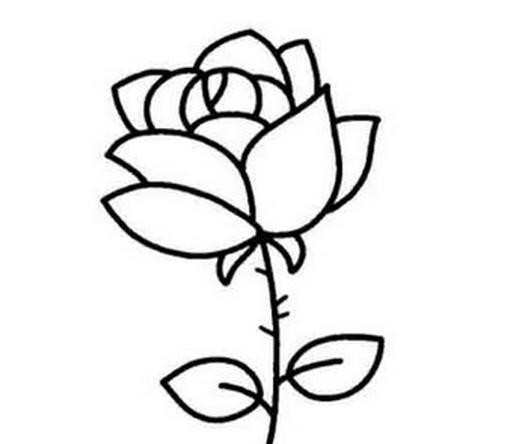
\includegraphics[width=1.5cm,height=2cm]{1.jpg}



假设喜欢你的ta又给了你另一支玫瑰

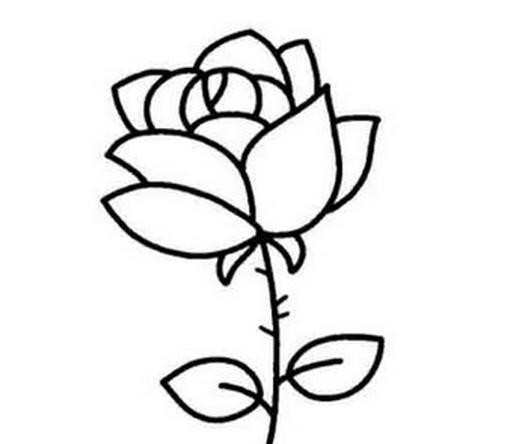
\includegraphics[width=1.5cm,height=2cm]{1.jpg}
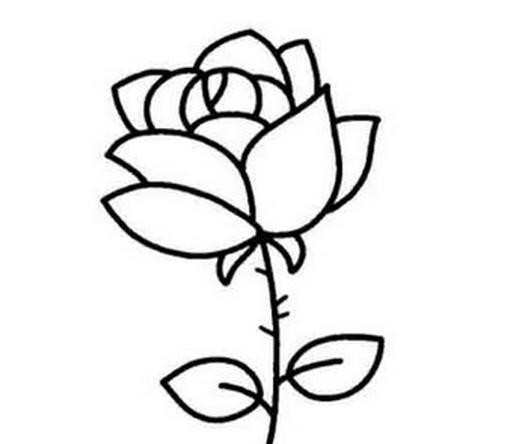
\includegraphics[width=1.5cm,height=2cm]{1.jpg}



现在,数一下你所拥有的玫瑰数量,你会得到结果是两支。也就是说一支玫瑰加一支玫瑰等于两支玫瑰,也就是一加一等于二。$$1+1=2$$

这就是算数的运算方法了。


那么,现在你已经对算数的基本原理有了一定的了解,就让我们来看一看下面两类简单的练习题,来把我们刚刚学到的知识运用到实践中吧。
\newline
\newline
\fbox{\textbf{试试看!}}

\subsection*{\leftline{1}}

(1)利用正交变换,证明Poisson公式$$\iint_{x^{2}+y^{2}+z^{2}=1}f(ax+by+cz)\mathrm{d}\sigma=2\pi\int_{-1}^{1}f(\sqrt{a^{2}+b^{2}+c^{2}}t)\mathrm{d}t$$


(2)证明$$\left|\iint_{x^{2}+y^{2}+z^{2}=1}f(mx+ny+pz)\mathrm{d}\sigma\right|\leq 2\pi M$$
其中$m^{2}+n^{2}+p^{2}=1$,$f(t)$在$|t|<1$是连续可微函数,$f(-1)=f(1)=0$,$M=\mathrm{max}|f'(t)|$.(提示,先利用Poisson公式化为定积分后再利用分部积分)

(3)证明:
$$\iiint_{x^{2}+y^{2}+z^{2}\leq1}f\left(\frac{ax+by+cz}{\sqrt{x^{2}+y^{2}+z^{2}}}\right)\mathrm{d}x\mathrm{d}y\mathrm{d}z=
\frac{2}{3}\pi\int_{-1}^{1}f(\sqrt{a^{2}+b^{2}+c^{2}}t)\mathrm{d}t$$
(提示:将球$x^{2}+y^{2}+z^{2}\leq1$分为无限多个薄球壳$x^{2}+y^{2}+z^{2}=r^{2},r\in [0,1]$的和,对于每一个薄球壳$x^{2}+y^{2}+z^{2}=r^{2}$使用Poisson公式化为定积分,再将所有的薄球壳的曲面积分加起来,即对$r$从0到1积分)

\subsection*{\leftline{2}}

有这样一类题,经常给出闭合曲线的外法线方向,然后用这个方向和其他的方向的夹角的三角函数作为被积函数来计算曲线(面)积分,解决这一类问题的关键就是将给三角函数转化为曲线的正切线和x,y轴夹角的余弦值或曲面的正法线和x,y,z轴夹角的余弦值,进而转化为第二类积分,用green或gauss即可算出.
\newline
\newline
\indent\textbf{例1:}
设$C$为光滑闭曲线,用$\bm{n}$表示$C$上各点处的单位外法向量,设$\bm{a}$是一个固定的单位向量,求证:
$$\int_{C}\mathrm{cos}(\bm{a,n})\mathrm{d}s=0$$

\textbf{思路分析:}

解决这样的题目要搞清楚对于一个曲线,法向量和切向量和坐标轴之间的夹角的关系,下文用$(\bm{a},\bm{b})$表示向量$\bm{a}$和$\bm{b}$的夹角,用$\bm{i},\bm{j},\bm{k}$各表示x,y,z正半轴方向的单位向量.

\begin{figure}[!h]
  \centering

  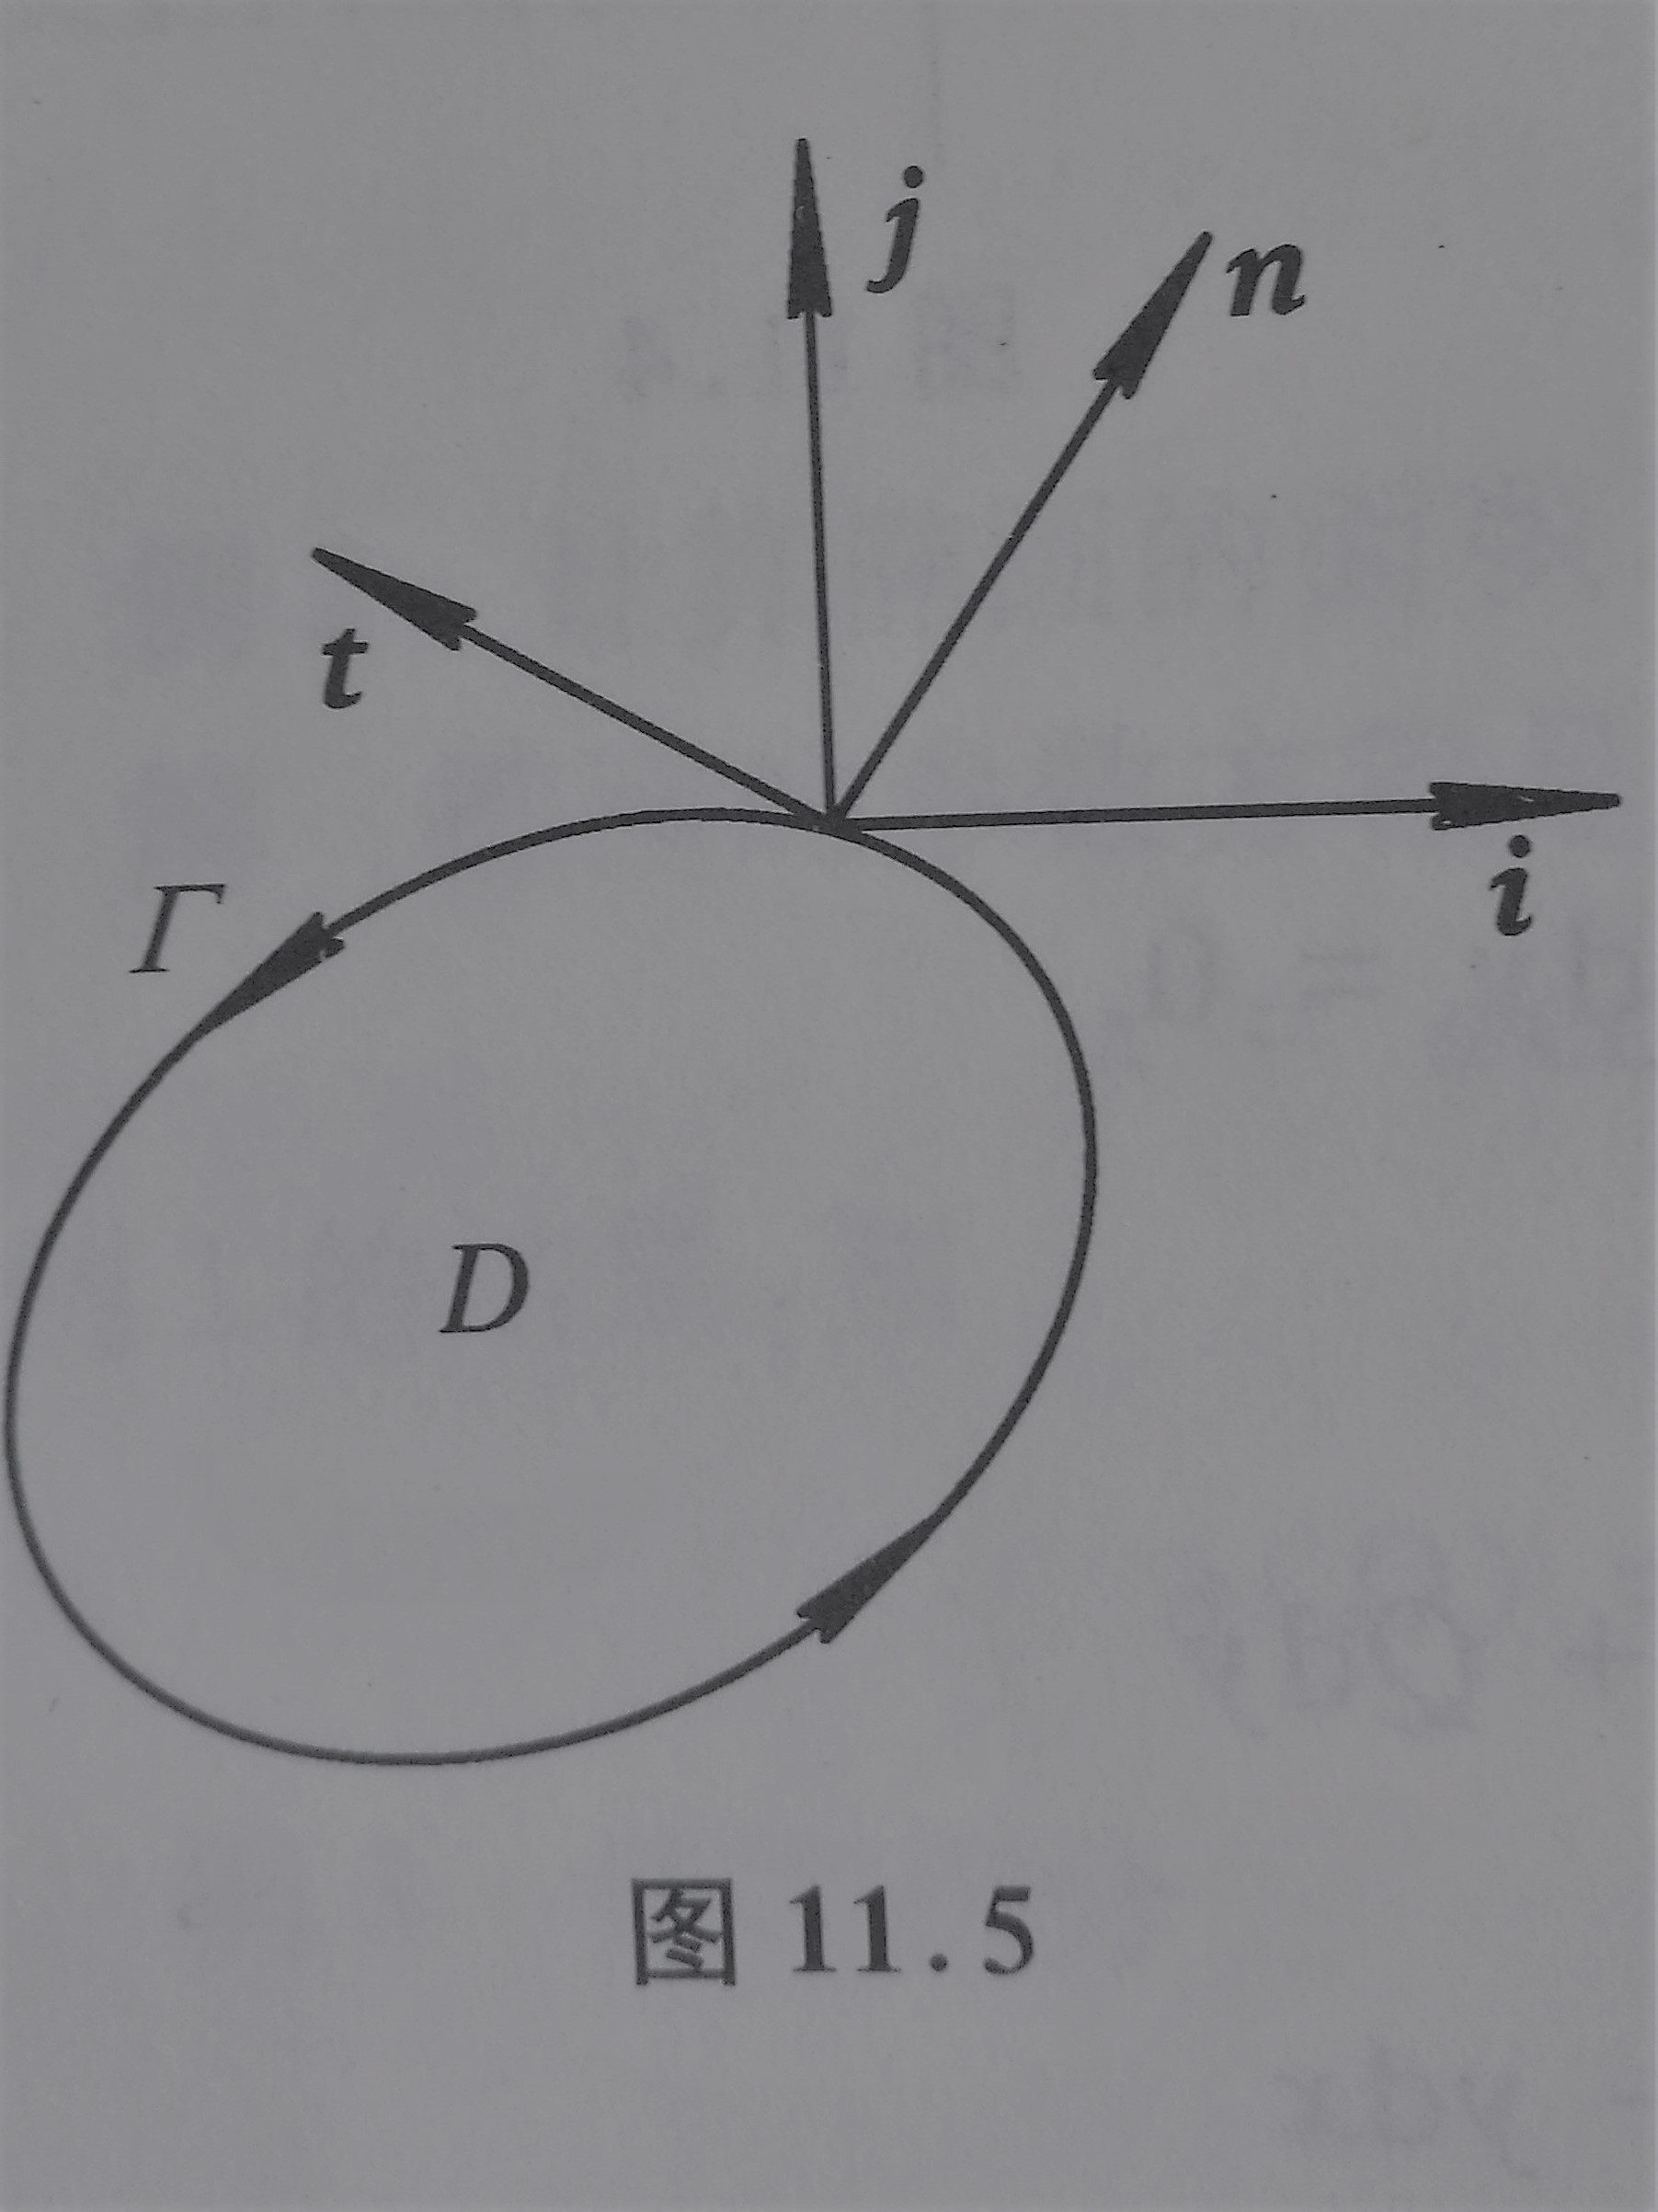
\includegraphics[width=5cm]{5.jpg}\\

\end{figure}

不妨设$\bm{a}=(m,n),m^{2}+n^{2}=1$,由上图,单位外法向量$\bm{n}$在x轴方向的分量为$|\bm{n}|\mathrm{cos}(\bm{n},\bm{i})=\mathrm{cos}(\bm{n},\bm{i})$(因为$\bm{n}$是单位向量),同理$\bm{n}$在y轴方向的分量为$\mathrm{cos}(\bm{n},\bm{j})$,所以可以求得$\bm{n}=(\mathrm{cos}(\bm{n},\bm{i}),\mathrm{cos}(\bm{n},\bm{j}))$,利用向量的点乘
\begin{align}
\mathrm{cos}(\bm{a,n})&=\frac{\bm{a}\cdot\bm{n}}{|\bm{a}|\cdot|\bm{n}|}&\nonumber\\
&=\bm{a}\cdot\bm{n}&\nonumber\\
&=m\mathrm{cos}(\bm{n},\bm{i})+n\mathrm{cos}(\bm{n},\bm{j})
\end{align}

由于要利用green公式,就必须转化为第一型曲线积分,回想起第一型曲线积分的转化,需要有切向量和x,y正半轴的夹角的余弦值.但是这里我们只有法向量和x,y正半轴夹角的余弦值
$\mathrm{cos}(\bm{n},\bm{i}),\mathrm{cos}(\bm{n},\bm{j})$,所以需要转换.

继续研究上图,设$\bm{t}$为正切向量,由于切向量和法向量垂直,x轴和y轴垂直,即$(\bm{n,i})+(\bm{n,j})=(\bm{n,j})+(\bm{t,j})=\pi/2$,所以有$(\bm{n,i})=(\bm{t,j})$,同理由于$(\bm{n,i})+(\bm{n,j})+(\bm{t,j})=(\bm{t,i}),(\bm{n,i})+2(\bm{n,j})+(\bm{t,j})=\pi$,两式相减有$(\bm{n,j})=\pi-(\bm{t,j})$.即
\begin{eqnarray}\nonumber
\begin{cases}
&\mathrm{cos}(\bm{n,i})=\mathrm{cos}(\bm{t,j})\\
&\mathrm{cos}(\bm{n,j})=\mathrm{cos}(\pi-(\bm{t,i}))=-\mathrm{cos}(\bm{t,i})
\end{cases}
\end{eqnarray}
带入到$(1)$中这样就能转化为切向量和坐标轴的夹角的余弦值,然后变为第二型积分就简单许多了
\begin{align}
\mathrm{cos}(\bm{a,n})\mathrm{d}s&=(m\mathrm{cos}(\bm{n},\bm{i})+n\mathrm{cos}(\bm{n},\bm{j}))\mathrm{d}s\nonumber\\
&=(m\mathrm{cos}(\bm{t,j})-n\mathrm{cos}(\bm{t,i}))\mathrm{d}s\nonumber\\
&=m\mathrm{d}y-n\mathrm{d}x\nonumber
\end{align}
再用green容易证明积分为0

\textbf{这道题的关键就是}将向量$\bm{a,n}$都写成坐标分量的形式,然后用公式$$\mathrm{cos}(\bm{a,n})=\frac{\bm{a}\cdot\bm{n}}{|\bm{a}|\cdot|\bm{n}|}$$这样就将难以处理的$\bm{a}$和$\bm{n}$的夹角转化为了$\bm{n}$ 和各个坐标轴的夹角.
\newline
\newline
\indent\textbf{练习1:}设$\Omega$是一闭域,向量$\bm{n}$是$\partial \Omega$的单位外法向量,$\bm{a}$是一个固定的向量.求证:
$$\iint_{\partial \Omega}\mathrm{cos}(\bm{a,n})\mathrm{d}\sigma=0$$
(提示:由于三维曲面的切向量不唯一,所以题目给方向的时候对于曲面只给法向量,又因为转化为第二型曲面积分时用的也是法向量和x,y,z正半轴夹角的余弦值,所以在一定程度上三维情形比二维的要简单.对于本题来讲只需要将$\mathrm{cos}(\bm{a,n})$转化为$\mathrm{cos}(\bm{n,i}),\mathrm{cos}(\bm{n,j}),\mathrm{cos}(\bm{n,k})$的组合即可,不需要考虑切向量和法向量的转换.)
\newline
\newline
\indent\textbf{练习2:}设$C$为二维光滑闭曲线,用$\bm{n}$表示$C$上各点处的单位外法向量,用$\sigma(D)$表示闭合曲线$C$围成的区域$D$的面积,证明:
$$\int_{C}(x\mathrm{cos}(\bm{n,i})+y\mathrm{cos}(\bm{n,j}))\mathrm{d}s=2\sigma(D)$$
\newline
\newline
\indent\textbf{例2:}
设$C$是一光滑闭曲线,$C$所围的区域为$D$,$(a,b)$是不在曲线上的一个定点,曲线上任意一点$(x,y)$的外法向量为$\bm{n}$,记$\bm{r}=(x-a,y-b)$,证明:
\begin{eqnarray}
\int_{C} \frac{\mathrm{cos}(\bm{r,n})}{|\bm{r}|}\mathrm{d}s=
\begin{cases}
2\pi&(a,b)\in D,\\
0&(a,b)\notin D.
\end{cases}
\end{eqnarray}

\textbf{思路分析:}
同例1一样的方法可以得到
\begin{eqnarray}\nonumber
\begin{cases}
&\mathrm{cos}(\bm{n,i})=\mathrm{cos}(\bm{t,j})\\
&\mathrm{cos}(\bm{n,j})=\mathrm{cos}(\pi-(\bm{t,i}))=-\mathrm{cos}(\bm{t,i})
\end{cases}
\end{eqnarray}根据$\bm{r}=(x-a,y-b),\bm{n}=(\mathrm{cos}(\bm{n,i}),\mathrm{cos}(\bm{n,j}))$计算出
\begin{align}
\frac{\mathrm{cos}(\bm{r,n})}{|\bm{r}|}\mathrm{d}s&=\frac{(x-a)\mathrm{cos}(\bm{n,i})+(y-b)\mathrm{cos}(\bm{n,j})}{|\bm{r}|^{2}}\mathrm{d}s\nonumber\\
&=\frac{(x-a)\mathrm{cos}(\bm{t,j})-(y-b)\mathrm{cos}(\bm{t,i})}{|\bm{r}|^{2}}\mathrm{d}s\nonumber\\
&=\frac{(x-a)\mathrm{d}y-(y-b)\mathrm{d}x}{(x-a)^{2}+(y-b)^{2}}\nonumber
\end{align}
有$\frac{\partial P}{\partial y}=\frac{\partial Q}{\partial x}$

再用green,即可得证.(注意,当$(a,b)\in D$时在点$(a,b)$处偏导数不连续,不能用green,所以要挖去一个半径足够小的圆$(x-a)^{2}+(y-b)^{2}\leq \varepsilon^{2}$,对剩余部分使用green, 对于圆上的积分用其他方法计算)
\newline
\newline
\indent\textbf{练习1:}设$\partial \Omega$是一光滑闭曲面,$\partial\Omega$所围的区域为$\Omega$,$(a,b,c)$是不在曲面上的一个定点,曲线上任意一点$(x,y,z)$的外法向量为$\bm{n}$, 记$\bm{r}=(x-a,y-b,z-c)$, 证明:
\begin{eqnarray}
\iint_{\partial\Omega} \frac{\mathrm{cos}(\bm{r,n})}{|\bm{r}|^{2}}\mathrm{d}\sigma=
\begin{cases}
4\pi&(a,b,c)\in \Omega,\\
0&(a,b,c)\notin \Omega.
\end{cases}
\end{eqnarray}
(提示:转化为第二型积分后用gauss,对于(a,b,c)是否在$\Omega$内要分类讨论)
\newline
\newline
\indent\textbf{练习2:}设$\Omega$为一闭区域,向量$\bm{n}$是$\Omega$的边界$\partial \Omega$的单位外法向量,点$(a,b,c)\notin\partial\Omega$,令$\bm{p}=(x-a,y-b,z-c)$,求证:
$$\iiint_{\Omega}\frac{\mathrm{d}x\mathrm{d}y\mathrm{d}z}{|\bm{p}|}=\frac{1}{2}\iint_{\partial \Omega}\mathrm{cos}(\bm{p,n})\mathrm{d}\sigma$$
\end{document}
